\chapter{Introduction} % Main chapter title

\label{ChapterIntroductionSCA}

\section{Notations and Probability and Statistics Recalls}\label{sec:notations}
\paragraph*{Basic Notations.}
In this thesis we use calligraphic letters as $\mathcal{X}$ to denote
sets, the corresponding upper-case letter $X$ to denote random variables (random
vectors $\vec{X}$ if with an arrow) over $\mathcal{X}$, and the corresponding
lower-case letter $x$ (resp. $\vec{x}$ for vectors) to denote realizations of
$X$ (resp. $\vec{X}$). The cardinality of a set $\mathcal{X}$ is denoted by $\lvert\mathcal{X}\rvert$. Matrices will be denoted with bold capital letters. When the vectors' orientation minds, they are understood as column vectors. The
$i$-th entry of a vector $\vec{x}$ is denoted by $\vec{x}[i]$, while the transposed of a vector $\vec{x}$ is denoted as $\vec{x}^\intercal$. We will use the transposed mark to refer to row vectors $\vec{x}^\intercal$. In general the $i$th observation of a random vector $X$ will be denoted by $x_i$. Observations will sometimes be grouped into datasets $\setData=\{x_1,\dots, x_N\}$. Throughout this thesis, a finite set $\sensVarSet = \{\sensVarValue{1}, \dots, \sensVarValue{\nbClasses}\}$ will be often considered: it will always denote the possible values for a \emph{sensitive variable} $\sensRandVar$ (see later). Its elements are sometimes encoded via a so-called \emph{one-hot-encoding}: to each element $\sensVarValue{j}$ a $\numClasses$-dimensional vector  $\sensVarOneHot{j}$ is associated,
with all entries equal to $0$ and the $j$-th entry equal to $1$: $\sensVarValue{j}
\rightarrow \sensVarOneHot{j} = (0,\ldots , 0,\underbrace{1}_{j},0,\dots,0)$. We will denote by $\sensVarGenValue$ a generic element of $\sensVarSet$, when useless to specify its index $\sensVarValue{i}$ for the context.

\paragraph*{Probability Notations.}
The probability of a random variable $X$ taking value in a subset $\mathcal{U}\in\mathcal{X}$ is denoted by $\prob(X\in\mathcal{U})$, or simply by $\prob(\mathcal{U})$ if not ambiguous. When $\mathcal{U}$ is reduced to a singleton $\mathcal{U}=\{x\}$ the same probability is denoted by $\prob(X=x)$ or simply by $\prob(x)$ if not ambiguous. If $X$ is a discrete variable $\pdf_X$ denotes its probability mass function (pmf for short), such that $\prob(X\in\mathcal{U})=\sum_{x\in \mathcal{U}}\pdf_X(x)$. The same symbol $\pdf_X$ is used to denote the probability density function (pdf for short) if $X$ is a continuous variable, such that $\prob(X\in \mathcal{U}) = \int_{\mathcal{U}}\pdf_X(x)dx$, for $[a,b]\subset\mathcal{X}$. 
The symbol $\esper[f(X)]$, or equivalently $\esper_X[f(X)]$, denotes the expected value of a function $f$ of the random value $X$, under the distribution of $X$. In the same way, symbols $\var(X)$ and $\var_X(X)$ denote the variance of $X$.

When two random variables $X$ and $Y$ are considered, their joint probability is denoted by $\prob(X=x,Y=x)$, or simply by $\prob(x,y)$ if not ambiguous, and their joint probability density (or mass) function is denoted by $\pdf_{X,Y}(x,y)$. The conditional probability of $X$ assuming the value $x$ given an outcome $y$ for $Y$ is denoted by $\prob (\given{X=x}{Y=y})$, or simply by $\prob(\given{x}{y})$ if not ambiguous. The conditional probability density (or mass) function of $X$ given an outcome $y$ for $Y$ is denoted by $\pdf_{\given{X} {Y=y}}(x)$. Finally, the covariance of the two variables is denoted by $\cov(X,Y)$.\\


\paragraph*{Bayes' Theorem.}
We recall some basic probability rules. For every $x\in\mathcal{X}$ and for every $y\in\mathcal{Y}$ we have what follows:
\begin{itemize}
\item \emph{Symmetry of joint probabilities: } $\pdf_{X,Y}(x,y)=\pdf_{Y,X}(y,x)$;
\item \emph{Marginal probabilities from joint ones: } $\pdf_X(x) = \sum_{Y=y}\pdf_{X,Y}(x,y)$ (where the sum has to be intended as an integral if $Y$ is a continuous variable);
\item \emph{Product rule: } $\pdf_{X,Y}(x,y) = \pdf_{\given{Y}{X=x}}(y)\pdf_{X}(x)$;
\end{itemize} 
These rules are sufficient to demonstrate, in the case of discrete random variables $X,Y$, a key stone of probability theory, the Bayes' theorem: 
\begin{equation}
\pdf_{\given{X}{Y=y}}(x) = \frac{\pdf_{\given{Y}{X=x}(y)}\pdf_{X}(x)}{\pdf_{Y}(y)} \mbox{ ;}
\end{equation}
the marginal probability function $\pdf_X$ is referred to as \emph{prior} probability of $X$, and describes the distribution of $X$ without taking into account the variable $Y$. The conditional probability $\pdf_{\given{X}{Y=y}}$ is referred to as \emph{posterior} probability of $X$, and gives the distribution of $X$ once the outcome $y$ of $Y$ is taken into account. Notions of measure's theory are needed to show that Bayes' theorem is valid and keeps unchanged in case of continuous random variables and in cases in which one of the two involved variables is discrete and the other one is continuous. The interested reader might refer to \cite{feller2008introduction}. 

\paragraph*{The Gaussian distribution.}
The Gaussian or normal distribution is a widely used model for the distribution of continuous variables. We use the symbol $X\sim\mathcal{N}(\mu,\sigma^2)$ to denote a random variable $X$ that follows a Gaussian distribution with parameters $\mu\in\mathbb{R}$ and $\sigma^2\in\mathbb{R}^{+}$. For a $D$-dimensional random vector $\vec{X}$ we use the symbol $X\sim\mathcal{N}(\mumumu,\Sigma)$ to denote a vector that follows a multivariate Gaussian distribution with parameter $\mumumu\in\mathbb{R}^D$ and $\Sigma\in\mathbb{R}^{D\times D}$ positive-definite. The density of the Gaussian distribution is completely determined by the value of its two parameters. It is given by the following expressions, in unidimensional and multidimensional case: 
\begin{equation}
\pdf_X(x) = \frac{1}{\sqrt{2\pi\sigma^2}}\exp{-\frac{1}{2}\left(\frac{x-\mu}{\sigma}\right)^2}\mbox{ ,}
\end{equation}
\begin{equation}
\pdf_{\vec{X}}(\vec{x}) = \frac{1}{\sqrt{2\pi\det(\Sigma)}}\exp{-\frac{1}{2}\left(\vec{x}-\mumumu\right)^\intercal \Sigma^ {-1}(\vec{x}-\mumumu)} \mbox{ .}
\end{equation}
The expected value of a Gaussian distribution coincides with the parameter $\mu$ for the univariate case and with $\mumumu$ for the multivariate one. The parameter $\sigma^2$ coincides with the variance of the univariate distribution, while $\Sigma$ coincides with the covariance matrix of the multivariate one.

\paragraph*{Basics of Statistics.}
The word \emph{statistics}  refers to a branch of mathematics that aims to analyse, describe or interpret observed data. Differently, the word \emph{statistic} refers to any measure obtained applying a function to some observed data. Let $\setData = \{x_1,\dots,x_N\}$ be a dataset of observations of a random variable $X$. We might distinguish two sub-branches in statistics: the descriptive statistics, and the inferential statistics. In descriptive statistics data are described by means of more or less complex statistics (in the sense of measure), the most common of them being the \emph{arithmetic mean}: 
\begin{equation}
\overline{x} = \frac{1}{N}\sum_{i=1}^N x_i \mbox{ .}
\end{equation}

In inferential statistics data are considered as sample observation of random variables and the data analysis aims at modelling the distribution of such variables. Dealing with random variables, inferential statistics exploit the probability theory framework and theorems. Statistics of data (in the sense of measures) play an important role in inferential statistics as well, usually aiming to estimate some random variable parameters. In this case they are called \emph{estimators} and will be denoted by a hat: for example, $\esperEst[X]$  denotes an estimator for the expected value of $X$ and $\varEst(X)$ denotes an estimator for the variance of $X$. The most classical estimator for the expected value is the arithmetic mean $\overline{x}$. It has several valuable properties, for example it is \emph{unbiased}, in the sense that, considering it as a random variable, its expected value coincides with the true value of $\esper[X]$. Moreover, it is the \emph{maximum-likelihood} estimator under the Gaussian distribution: for data that are independent among each other and drawn from a Gaussian distribution,  the arithmetic mean of the observed data $\setData$ is the value for the parameter $\mu$ that maximises the probability of observing the data $\setData$. A common unbiased estimator for the variance is the following so-called sample variance: 
\begin{equation}
\varEst = \frac{1}{N-1}\sum_{i=1}^N(x_i-\overline{x})^2 \mbox{ ;}
\end{equation}
when the observed random variable  follows a Gaussian distribution, such an estimator differs from the maximum-likelihood one, in which the factor $\frac{1}{N-1}$ is substituted by $\frac{1}{N}$. In the same way, acting with Gaussian random vectors, the maximum-likelihood estimator of the covariance matrix is biased, and differs from the common unbiased one for a multiplicative factor. \\

Various approaches exist to make statistical inference. The two main ones are the frequentist approach and the Bayesian one. The frequentist inference is an approach that draws conclusions exclusively from sample data. It makes use of methodologies like the statistical hypothesis testing and the confidence interval, and in this thesis it is sometimes referred to as classical statistics. In the frequentist approach, parameters that define the distribution of the analysed random variable are priorly considered as fixed and unknown, and are estimated or tested on the sole basis of the observation of the sample data $\setData$. A second approach is the Bayesian inference, for which parameters that describe the analysed random variable are admitted to be probabilistic: in Bayesian inference, before the observation of sample data, the parameters have a prior distribution that reflects the knowledge and belief of the data-scientist about them. The observation of data leads to an update procedure, based on the Bayes' theorem, that allows such probability distribution of parameters to become more and more appropriate, each time exploiting the new available information. For both approaches, the maximum-likelihood is an optimal statistical principle and is widely exploited to choose parameters, in the frequentist approach, or to update parameters' probability distributions in the Bayesian one. Up-to-now the Bayesian inference has never explicitly influenced the Side-Channel Attack literature, nor we will use such a framework in this thesis. We leave this track opened for future works, briefly discussing its suitability for Side-Channel Attacks domain in Chapter~\ref{ChapterConclusions}.

\section{Introduction to Side-Channel Attacks}
%\subsection{Introduction}
%\subsubsection{Generalities: Grey-Box, Divide-and-Conquer}
Side-Channel Attacks (SCA) belong to the cryptanalysis domain, since they aim to breach cryptographic security systems. Usually their goal is to retrieve a secret variable of a cryptographic algorithm, typically a secret key. They distinguish from classic mathematical cryptanalysis techniques by the fact that they are based on information gained from the physical implementation of a cryptosystem, rather than theoretical weaknesses in the algorithms. 
The possibility to physically observe the electronic device that performs the cryptographic computations, allows Side-Channel Attacks to go beyond the cryptographic complexity that assures resistance against classical cryptanalysis strategies.  Indeed, no matter the size of the secret variables manipulated by the algorithm and the algebraic complexity of the encrypting/decrypting operations, an physical implementation of any algorithm always handles variables of a bounded size, that depends on the hardware architecture of the cryptographic device. For example, in an 8-bit architecture an AES with 128-bit-sized key will be necessarily implemented as multiple partial computations over 8-bit blocks of data. In classical cryptanalysis, the typical attacker model faces to a black-box that performs the cryptographic algorithm: an attacker may make queries to the black-box, asking for ciphertexts of given plaintexts or viceversa. The black-box acts as a function that output the asked value, but does not provide any information about partial computations. On the contrary, a side-channel attacker is said to face to a \emph{grey-box} model: he has a way to obtain noised information about partial computations. This allows him to perform a \emph{divide-and-conquer} strategy: if his goal is to retrieve the full 128-bit AES key, he will smartly divide his problem into the recovery of small parts of such keys at time, called \emph{key chunks},\footnote{or \emph{subkeys} when they coincide to a byte of key for the AES algorithm} making the complexity of the attack significantly drop. 

\subsection{An Overview}
Since the seminal paper by Paul Kocher in 1996 \cite{kocher1996timing}, side-channel analysis domain has developed fast, together with its flourish literature. Without being exhaustive, the last literature includes: proposals for new kind of exploitable signals, proposals for useful statistical tools, new attacks strategies and routines, analysis of side-channel vulnerabilities of well-specified cryptographic algorithms, side-channel countermeasures, formal proofs of countermeasures' security claims, discussions about tools and metrics to compare side-channel attacks and strategies, reports of real-case successful attacks, and a few attempts to unify the side-channel literature under some comprehensive frameworks. The contributions we present in this thesis may be resumed as proposals for statistical tools for some specific attack contexts. The aim of the following part of this section is not to provide a comprehensive state-of-the-art of the side-channel domain, but to provide the reader with the necessary concepts to understand such contributions, and get a view of the contexts in which they can provide improvements to the state-of-the-art. To this aim we propose a brief overview of the main properties that define and characterise a side-channel attack among others. To describe a side-channel attacks, we identified  the following characteristics: 
\begin{itemize}
\item the physical nature of the exploited signals,
\item the chosen sensitive variables,
\item the strategy family,
\item the \emph{shape} of the attack,
\item and the attacker knowledge.
\end{itemize} 

In the following sections we will briefly describe these points, dwelling on aspects that  mainly concern our contributions, \eg the \emph{advanced attack} strategy and the concept of \emph{profiing attack}. 

\subsection{Physical Nature of the Exploited Signals}\label{sec:physical_signals}
As already introduced in Sec.~\ref{sec:SCAintro}, a SCA may exploit signals obtained by the observation of different kind of \emph{side channels}. Mainly exploited physical quantities are the power consumption, the electromagnetic emanation, the elapsing time and the acoustic emanation. 

\subsection{Sensitive Variables}\label{sec:sensitive_variables}
Physical signals are acquired \via appropriate instrumentation, and collected into vectors called \emph{traces} (or \emph{acquisitions}). They will be denoted by $\vLeakVec_i$ and considered as observations of a random real vector $\vaLeakVec$, where each coordinate corresponds to a time sample of the acquired signal.  They are then interpreted as noisy observations of the intermediate variables handled by the device during the execution. An attacker is in particular interested to the so-called \emph{sensitive variables}:  they are quantities handled during the processing that depend somehow on a secret of the implementation, and not only on public variables, as a plaintext or an algorithm constant. Side-channel analysis acts clearing traces from noise, in such a way to determine with the highest possible precision the association between a trace (or a set of traces) and the value taken by the target \emph{sensitive variable} $\sensRandVar$ during its (their) acquisition. For an attack, a single or several sensitive variables may be targeted, and its/their algebraic relation with the secret key serves to complete the attack.  Actually, \emph{sensitive variables} would be more appropriately called \emph{sensitive targets}, since they might not be variable. Some typical examples of sensitive variables include: 


\begin{itemize}
\item $\sensRandVar = \keyRandVar$ with $\keyRandVar$ a secret subkey - this is the most direct choice for a sensitive target, nevertheless it is often not variable, since in some cases a device always manipulates the same key for a given embedded primitive. When the target is not variable we are performing a \emph{simple attack} (see Sec.~\ref{sec:simple});
\item a cryptographic variable that depends on a sufficiently small subkey and a part of a known input variable $\publicParRandVar$: $\sensRandVar = \sensFunction(\keyRandVar,\publicParRandVar)$ - this is the most classical choice to perform a so-called \emph{differential} or \emph{advanced} SCA (see \ref{sec:advanced});
\item any function of a cryptographic variable (ex: $\HW(\sensFunction(\keyRandVar,\publicParRandVar))$), where $\HW(\cdot)$ represents the Hamming weight operation, \ie the operation that counts the number of 1's in the binary string representing the entry. Sometimes, as for example we will see in Chapter~\ref{ChapterKernel} (see Sec.~\ref{sec:multiclass}) it can be interesting not to target a variable but a non-injective function of a variable as its Hamming weight; when the identity function is applied we are in the previous case;
\item an operation (ex: $\sensRandVar \in \{\mathrm{square}, \mathrm{multiply}\}$)
\item a register (ex: $\sensRandVar$ is the register used to store results of intermediate operations in a Montgomery ladder implementation of RSA)
\end{itemize}
In this thesis we will try as much as possible to abstract from the form of the sensitive variable, thinking of any entity $\sensRandVar$ that assumes values in a finite set $\sensVarSet$ and whose value permits an attacker to make inference on a secret of the implemented algorithm.

\subsection{The Strategy Family}\label{sec:strategies}
The wide range of attack strategies, together with their still-evolving taxonomy, makes the task of group attack strategies very hard. We propose here a simplified grouping into three strategy families: 
\begin{itemize}
\item  the \emph{Simple Attacks},
\item the \emph{Collision Attacks}, 
\item the \emph{Advanced Attacks}.
\end{itemize}  
We highlight the fact that such a grouping is not sharp and impermeable in literature. 


\subsubsection{Simple Attacks}\label{sec:simple}
\begin{figure}
\centering
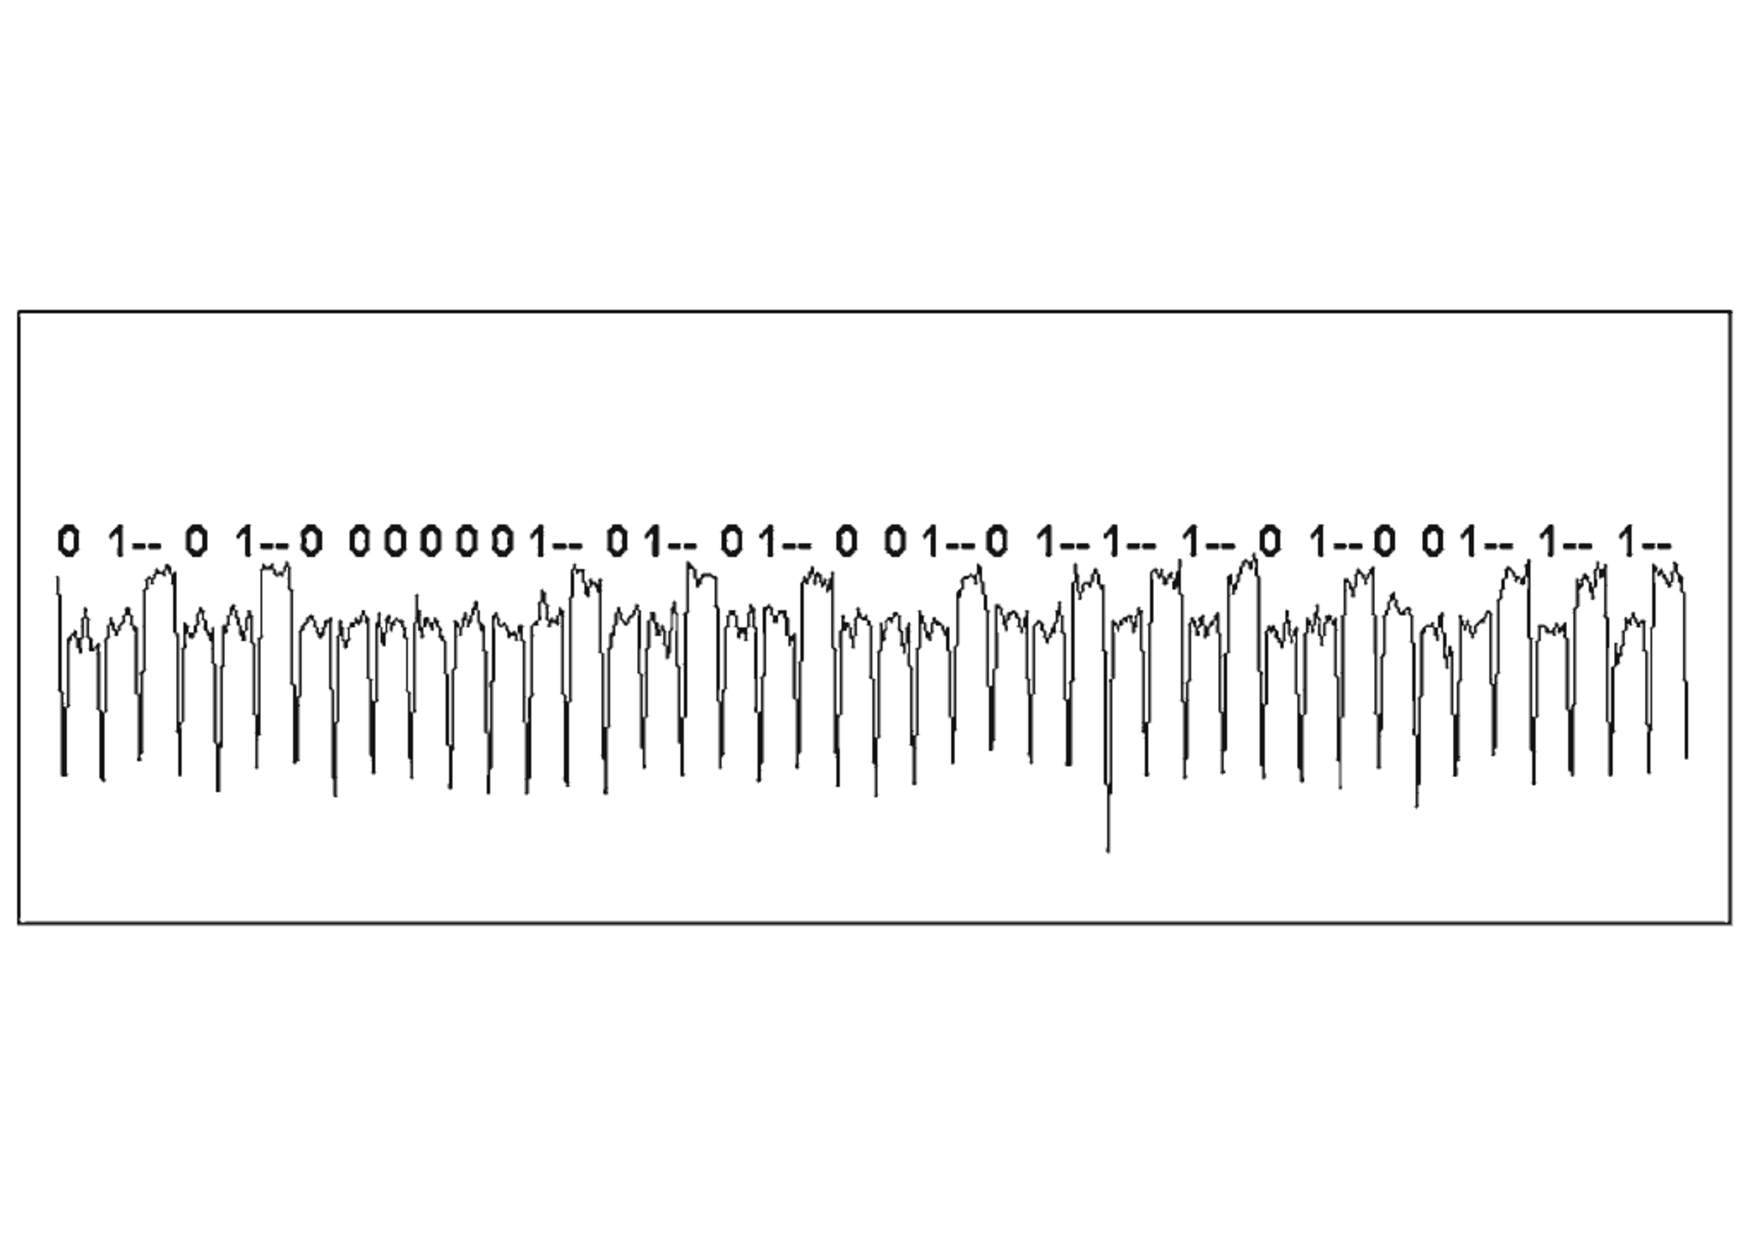
\includegraphics[width=0.7\textwidth]{../Figures/SPA_SM_kocher_2011.pdf} 
\caption{Simple attack against RSA implementation. Source: \cite{kocher2011introduction}.}\label{fig:SPA}
\end{figure}

In simple attacks, the relevant information is obtained directly from the observation of trace pattern, without necessarily apply statistical tools and often at the naked eye. Such a direct analysis is sometimes referred to as \emph{Simple Power Analysis} (SPA). The sensitive variable coincides in general with the secret key (or a chunk of it). Typical targets for SPA attacks are cryptographic devices in which some operations requires variable timing instructions, or in which the execution path depends on the key. For example, considering software-implementation, branching to different instructions may occur when a secret key chunk has a specific value, in general dealing with operations as comparisons, multiplications or exponentiations. A typical example of leaks allowing simple attack is depicted in Fig.~\ref{fig:SPA}: the depicted trace shows a sequence of squares and multiplications performed by a device computing modular exponentiation to implement the RSA algorithm. Multiplications consume more than squares and patterns are recognizable to the eye. The sequence of patterns directly reveals the secret key. A characteristic of simple attacks is that they do not require in general to observe the variation of the side-channel signals under the variation of the algorithm entries, thus they are sometimes referred to as \emph{one-trace attacks}, since the observation of a single trace may be sufficient to perform them. In literature the terms \emph{simple attacks} and \emph{one-trace attacks} are sometimes considered equivalent, as \eg in \cite{exponent2012rosetta}. Anyway, we aim to include in the \emph{simple attacks} family those attacks for which many observations are acquired with fixed entry parameters and by consequence in which the observed leakage always corresponds to a fixed value of $\sensRandVar$. The attacker may exploit the several acquisitions in mainly two ways: he computes their average before performing the attack (as done for example in the simple attack proposed by Mangard in 2002 \cite{mangard2002simple}, and ameliorate in 2014 by Clavier \etal \cite{clavier2014simple}), aiming to reduce the noise influence, or he performs the attack of each acquisition (expecting each gives the same outcome) and then applies a function to the several outcomes (\eg majority vote) to guess the right label. We observe that this approach with several observations allows the attacker to reduce the noise impact, while observing many times the same variable. The relation between the variable and the key chunk being fixed (and being the identity, in general), he will not exploit algebraic relations to ameliorate his inference over the latter. In next chapter, Section~\ref{sec:TPE}, we will describe some classic example of machine learning task. Here we point out the fact a simple attacks exactly correspond to resolving a \emph{classification task} in side-channel context. 


\subsubsection{Collision Attacks}
Collision attacks were introduced by Schramm \etal in 2003 \cite{schramm2003new} as a side-channel generalisation of classic cryptanalysis collision attacks, typically used to break cryptographic hash functions. They deduct information about the secret key of a block cipher from the presence or the absence of an internal collision during the encryption (or decryption). A collision has to be intended as the fact that, while processing different inputs, an internal computation acts over the same operand, or outputs the same value. To perform a collision attack, the side-channel attacker is thus not required to interpret side-channel signals to perfectly understand which operation is executed and over which operands. The assumption is weaker: the attacker is supposed to be able to state if two signals (or portions of signals) correspond or not to the same operation. In the seminal work \cite{schramm2003new}, as in several further developments as \cite{ledig2004enhancing,schramm2004collision,bogdanov2007improved,bogdanov2008multiple}, sets of several acquisitions under well-chosen entries are exploited to establish, through statistical tools, \eg correlation estimators, whether a collision is present. In the same year 2003, Fouque and Valette \cite{fouque2003doubling} proposed a collision attack in a context declared by authors more favourable than block ciphers, \ie operations like modular exponentiation.\footnote{or scalar multiplication in the elliptic curve setting} In this context, authors proposed an attack strategy based on the observation and comparison of only two acquisitions. In analogy with simple attacks, often labelled as \textquotedbl one-trace\textquotedbl , correlation attacks are thus somehow categorised as \textquotedbl two-traces\textquotedbl attacks, even if this connotation is not always pertinent. In particular, collisions might be searched in different parts of the same trace, \ie in a \emph{horizontal} fashion (see Sec.~\ref{sec:form}), leading collision attacks applicable with a single trace, \eg as done in \cite{clavier2010horizontal} to attack an RSA implementation protected against simple attacks. However, as we highlighted at the beginning of this section, the terms about side-channel strategy are still not unambiguous in literature, for example, in the summarising work proposed by Kocher \etal in 2011 \cite{kocher2011introduction}, collision attack are considered as a variant of simple attacks. Again in analogy with simple attacks, and in the same way we observed that simple attacks perfectly declines the machine learning task of classification, we observe that collision attacks are in a strong analogy with another classical machine learning task, \ie the \emph{verification task}, that will be as well introduced in Sec.~\ref{sec:TPE}.

\subsubsection{Advanced Attacks} 
In contrast to the \emph{Simple Power Analysis}, enabling simple attacks when large-scale side-channel variations depend on secret values and low noise is present, the so-called \emph{Differential Power Analysis} (DPA) refers to techniques that exploit  a statistical approach to reveal key-dependent lower-scale side-channel variations. DPA techniques enables the so-called \emph{advanced attacks}. With respect to simple attacks, advanced attacks do not require a detailed knowledge of the implementation details, and are able to succeed even dealing with acquisitions containing a considerable amount of noise. The term \emph{Differential} refers to the fact that the approach exploits the small differences in the behaviour of the device while handling varying sensitive variable. By consequence, in contrast to simple attacks,  several acquisition have to be observed to perform an advanced attack, under varying values for the chosen sensitive variable. Intuitively, the small differences are get larger by means of averaging over an eventually considerable amount of acquisition. As much noise hides informative differences, as many acquisitions are needed to clear it and make information emerge. Interestingly, the first DPA tool (or \emph{distinguisher}, as will be introduced below) proposed to perform an advanced attack were the so-called \emph{Difference of Means} (DoM) (the method were proposed by \cite{kocher1999differential}, but the name given by \cite{Chari2003}),  in which differences where exactly looked for by subtraction. A more precise description of the advanced attacks is provided in Sec.~\ref{sec:advanced}.\\



\subsection{The Shape of the Attack}
\begin{figure}
\centering
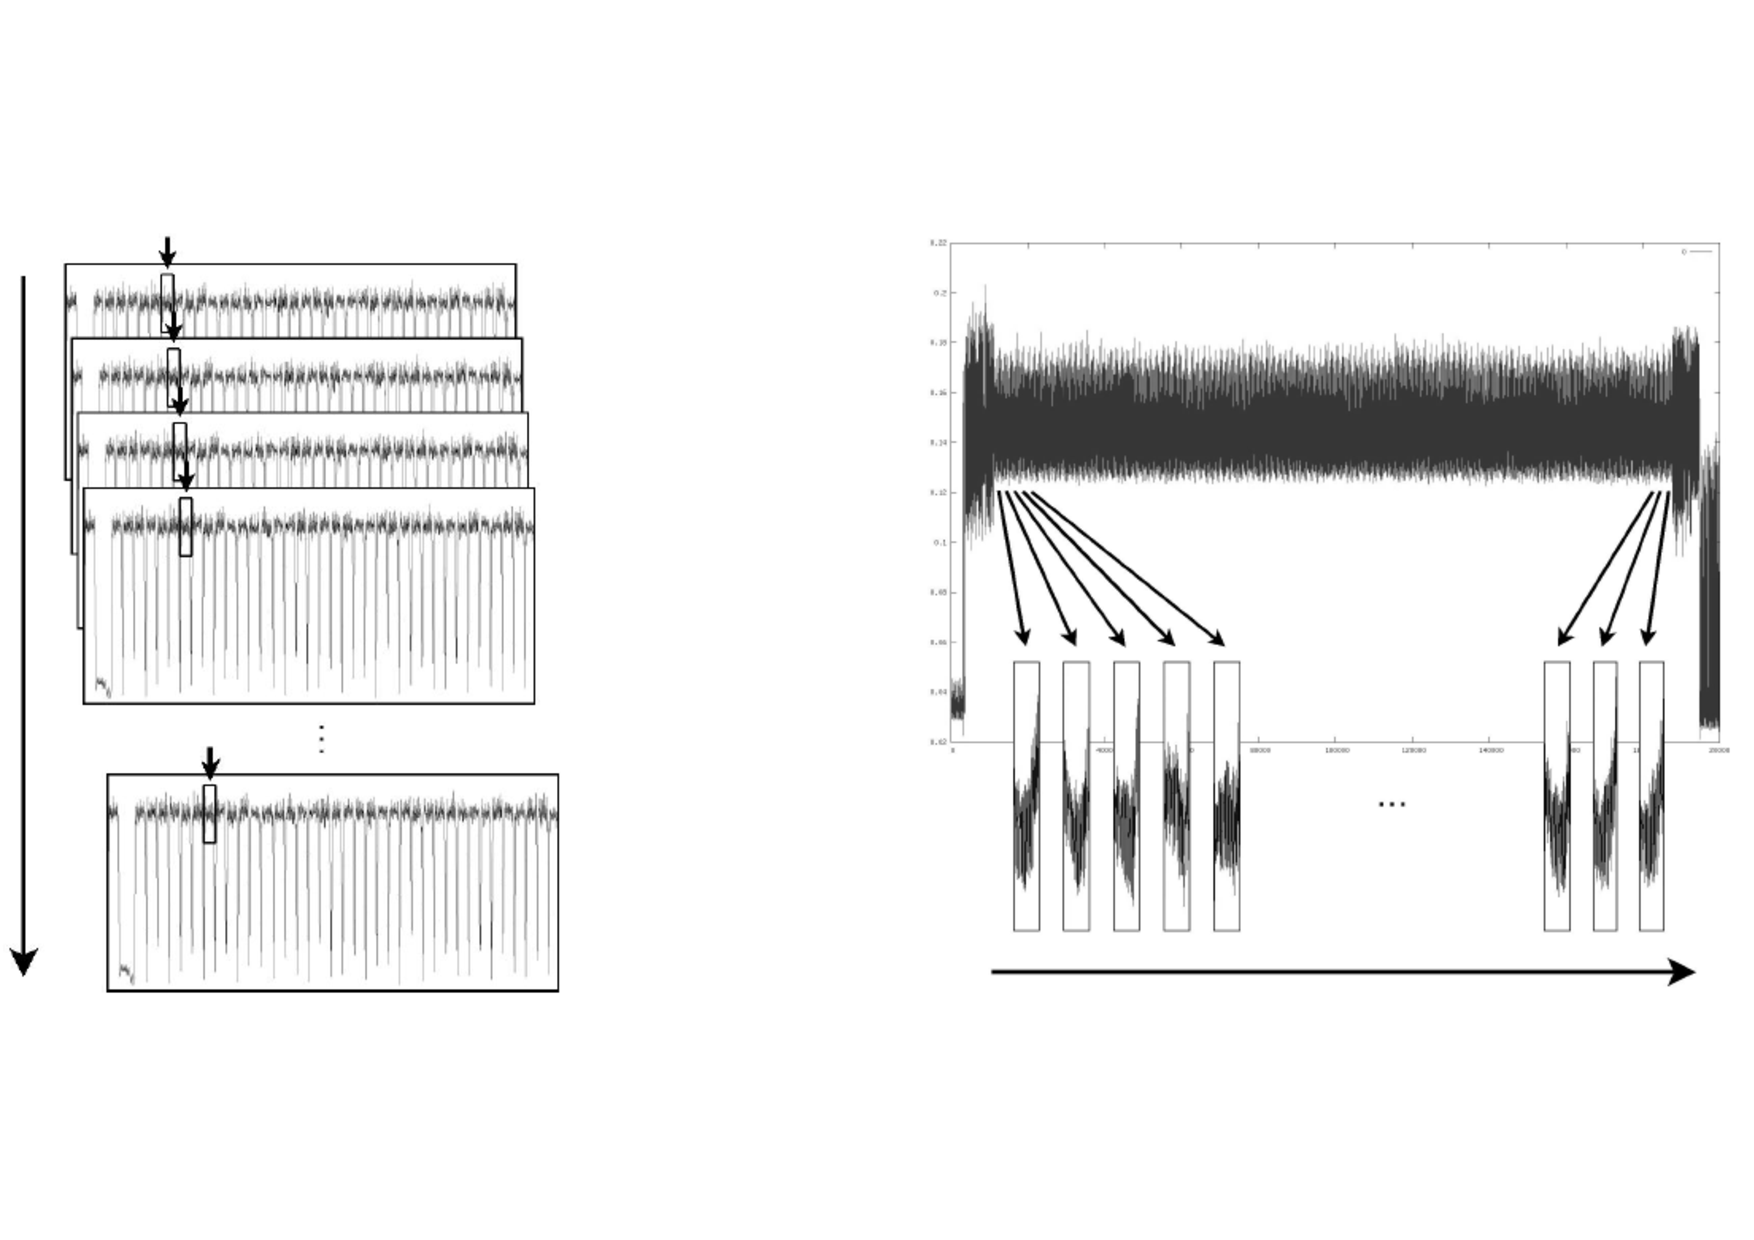
\includegraphics[width=0.7\textwidth]{../Figures/horizontal_vertical.pdf} 
\caption[Vertical and horizontal attacks.]{Vertical (left) and horizontal (right) attack. Source: \cite{clavier2010horizontal}.}\label{fig:vert_hor}
\end{figure}
In \cite{clavier2010horizontal} a distinction between \emph{vertical} and \emph{horizontal} attacks is proposed, adopted in several posterior publications, \eg \cite{bauer2013horizontal} which proposes horizontal approach to attack secure implementations of RSA, or \cite{battistello2016horizontal} in which an horizontal approach is used to counteract a \emph{masking} countermeasure (see Sec.~\ref{sec:masking}). \emph{Vertical attacks} are intended as techniques analysing the same sample time regions of several side-channel traces, while \emph{horizontal attacks} analyse many portions of a single trace, as depicted in Fig.~\ref{fig:vert_hor}. In typical scenarios,  horizontal attacks are associated to simple SCAs (see \eg Fig.~\ref{fig:SPA}), while vertical ones are associated to advanced SCAs. Collision attacks might be vertical or horizontal depending on whether collisions are looked for in a same execution or in more than one execution.  Anyway, simple attacks exploiting many acquisitions to reduce the noise impact have a vertical behaviour, and advanced attacks may be performed in an horizontal manner as done \eg in \cite{battistello2016horizontal}: this is possible observing that, in the attacked cryptographic algorithm, several different intermediate computations depend on the same sensitive variable, thus the last variable may be observed varying by observing those computations. This kind of approach exploits the algebraic dependency between several intermediate. This concept is at the basis of another special class of SCAs, the so-called \emph{Algebraic Side-Channel Attacks} \cite{ASCA,renauld2009algebraic,Oren:2013,Oren2014,soft}. The Algebraic SCAs combine profiling SCA strategies (see \ref{sec:profilingSCA}) to classical cryptanalysis techniques, \ie without necessarily exploiting divide-and-conquer strategy, but retrieving the whole key secret at once solving algebraic systems in which plaintexts, chipertext and potentially all observable intermediate variable are involved. They act in an horizontal manner, and may need more than one acquisition to get a unique key candidate. The nice notion of \emph{rectangular} attacks, introduced in \cite{bauer2013horizontal}, and denoting attacks that both exploit several portions of a signal, but taking advantage of several acquisitions, probably describes the great majority of the modern attacks. 


\subsection{The Attacker Knowledge}
Many aspects of the attacker knowledge on the target implementation may influence his approach. For example the level of knowledge of implementation details may allow or not to perform a simple attack. In an evaluation context, we may assume that an evaluator has open access to implementation details. Nevertheless, we are here interested in distinguish two particular attack scenarios that influence his knowledge about the physical behaviour of the device: the \emph{profiling} and \emph{non-profiling} attacks.
As anticipated in Sec.~\ref{sec:this_thesis_objectives}, when an open sample of the attacked device is available to make a prior characterisation of the leaking signals of a device, we talk about \emph{profiling} attacks. When this is not the case, we talk about \emph{non-profiling} attacks. Profiling attack are the mainly concern of this thesis, and are deeper introduced in Sec.~\ref{sec:profilingSCA}. \\


\section{Efficiency of the SCAs}\label{sec:metrics}
In order to measure the efficiency of a side-channel attack, different security metrics have been proposed, the most exploited being the \emph{success rate of order} $\orderRate$ ($\SR_\orderRate$) and the \emph{guessing entropy} (GE). Referring to the formalization proposed by \cite{unifiedFramework}, a key recovery side-channel attack outputs a vector of key candidates,\footnote{In this thesis we will always target a key chunk and we will use such metrics to evaluate the efficiency of an attack in recovering such key chunks. When a full-key recovery attack is run, some algorithms to merge key chunks' outcomes and obtain the full key enumeration and a complete key rank estimation are deployed. This domain is out the scope of this thesis.} called {\em guessing vector} $\guessingVector = \left[\guessingVector[1], \dots, \guessingVector[{\lvert \keyVarSet \rvert}]\right]$, in which such candidates are sorted in decreasing order with respect to their likelihood after the attack phase. Being $\keyVar^\star$ the right candidate, its \emph{rank} is given by:
\begin{equation}
\mathrm{Rank}(\keyVar^\star) = i \mbox{ such that } \guessingVector[i] = \keyVar^\star \mbox{.}
\end{equation}

Then, the success rate of order $\orderRate$ of an attack is given by the probability for the right key candidate to be ranked among the first $\orderRate$ candidates: 

\begin{equation}
\SR_\orderRate = \prob[\mathrm{Rank}(\keyVar^\star)\leq \orderRate] \mbox{ .}
\end{equation}

The success rate of an attack is usually estimated empirically: the attack is repeated a large number of times, and the empirical $\SR_\orderRate$ is given by the ratio between the number of successes (attacks for which the right key is ranked among the first $\orderRate$ ones) and the total number of attacks. \\

The guessing entropy \cite{massey1994guessing} is defined as the expected rank of the right key: 
\begin{equation}
\guessingEntropy = \esper[\mathrm{Rank}(\keyVar^\star)]\mbox{ .}
\end{equation}

This is also generally estimated in an empirical way, by performing the attack many times independently, then computing the average of the obtained ranks. 



\section{Advanced Attacks}\label{sec:advanced}
An advanced attack can be summarised in the following five steps: 
\begin{itemize}
\item acquire side-channel traces $(\vLeakVec_i)_{i=1,\dots , \nbTraces}$ making entries $(\publicParVar)_{i=1,\dots,\nbTraces}$ vary,
\item choose a sensitive variable $\sensFunction(\keyRandVar,\publicParRandVar)$, 
\item define a \emph{leakage model}, \ie a function $\leakageModel(\sensRandVar)$ modelising the side-channel leakage for a given sensitive variable value (some examples are given in Sec.~\ref{sec:leakage_models}),
\item for every key chunk hypothesis $\keyVar \in \keyVarSet$ predict the side-channel leakage 
\begin{equation}
\leakageModel_{\keyVar,i} = \leakageModel(\sensFunction(\keyVar,\publicParVar_i)) \mbox{ ,}
\end{equation}
\item statistically compare the hypothetical predictions to the observed side-channel acquisitions, by means of a  \emph{distinguisher} $\distinguisher$ (see Sec.~\ref{sec:distinguishers}):
\begin{equation}
\distinguisher_{\keyVar} = \distinguisher((\vLeakVec_i)_{i=1,\dots , \nbTraces}, (\leakageModel_{\keyVar,i} )_{i=1,\dots , \nbTraces}) \mbox{ ,}
\end{equation}
\item deduce the key chunk candidate from scores $\distinguisher_{\keyVar}$, in general coinciding with the key hypothesis that maximises or minimises the scores.
\end{itemize}

\subsection{Leakage Models}\label{sec:leakage_models}
Classical leakage models are based on the fact that, in CMOS technology (which is used to realise the majority of existing integrated circuits), peaks of power consumption are observable when the output of the gates transition from either a \textquotedbl 0\textquotedbl to \textquotedbl 1\textquotedbl or a \textquotedbl 1\textquotedbl to \textquotedbl 0\textquotedbl logic state.  For an internal variable $\sensRandVar$, examples of classical leakage models $\leakageModel(\sensRandVar)$ are:
\begin{itemize}
\item \emph{mono-bit model}: the value of one bit of $\sensRandVar$,
\item\emph{Hamming weight model}: the Hamming weight $\HW(\sensRandVar)$,
\item \emph{Hamming distance model}: the Hamming distance between $\sensRandVar$ and another intermediate variable $\sensRandVar^\prime$, defined as $\mathrm{HD}(\sensRandVar,\sensRandVar^\prime) = \HW(\sensRandVar\oplus\sensRandVar^\prime)$, supposing \eg that one of the two variable overwrites the other into the same logic states (thus, the number of switches is counted),
\item \emph{linear model}: a linear combination of the bits of $\sensRandVar$, supposing that some states influence the power consumption more than other, 
\item \emph{identity model}: the value of $\sensRandVar$ itself.
\end{itemize} 

\subsection{Distinguishers}\label{sec:distinguishers}
The underlying core hypothesis of an advanced SCA is the following. Given a set of side-channel traces, \ie a set of realizations of a random variable $\vaLeakVec$, the attacker computes the realizations of a second random variable $\leakageModel_\keyVar$ per each key hypothesis. For the correct key hypothesis, the two random variables $\vaLeakVec$ and $\leakageModel_\keyVar$ are statistically dependent, while for the wrong key hypothesis they are independent (or at least \emph{apparently} independent, as pointed out in Rem.~\ref{rem:ghost}). The goal of a distinguisher is to detect the dependencies between the two random variables. Thus, the selected key candidate is the one that shows an higher dependency value between the  predicted leakages and the actual ones. 

\begin{remark}\label{rem:ghost}
Actually this vision is too strong: a dependency always exists between the wrong key candidate hypothetical leakages and the actual ones (and in literature it has been evidenced under the name of \emph{ghost peaks} in \cite{brier2004correlation}), but such a dependency is hard to detect statistically: deterministic functions that link wrong key hypothesis to the correct ones are those that define the cryptographic algorithm, thus in general algebraically complex and highly non-linear. For example, let us consider $\sensRandVar = \Sbox(\keyRandVar \oplus \publicParRandVar)$ as sensitive variable for an AES implementation, and choose in identity leakage model. Let $\keyStar$ be the right key chunk and $\hat{\keyVar}$ be a wrong candidate. The right leakage predictions $\leakageModel_{\keyStar, i} = \Sbox(\keyStar \oplus \publicParVar_i)$ and the wrong ones $\leakageModel_{\hat{\keyVar}, i} = \Sbox(\hat{\keyVar} \oplus \publicParVar_i)$ are linked by the following deterministic relation: 
\begin{equation*}
\leakageModel_{\hat{\keyVar}, i} = \Sbox(\Sbox^{-1}(\leakageModel_{\keyStar, i})\oplus \keyStar \oplus \hat{\keyVar}) \mbox{ ,}
\end{equation*}
implying that, if a statistical dependence exists between the random variables $\leakageModel_{\keyStar}$ and $\vaLeakVec$, then $\leakageModel_{\hat{\keyVar}}$ and $\vaLeakVec$ are statistically dependent, as well.
\end{remark}

Among the most popular side-channel distinguishers, many looks only for linear dependencies, \eg the Difference of Means (DoM) and the Correlation Power Analysis (CPA). The DoM is the one exploited in in \cite{kocher1999differential} with a mono-bit model (implying that $\leakageModel_\keyVar$ takes only two values, $0$ and $1$), then generalised for other leakage models in \cite{Rechberger2005}, under the name of Sum of Differences (SoD). It has the following form: 
\begin{equation}
\distinguisher^{DoM}_{\keyVar} = \esperEst[\given{\vaLeakVec}{\leakageModel_\keyVar = 0}] - \esperEst[\given{\vaLeakVec}{\leakageModel_\keyVar = 1}]   \mbox{ .}
\end{equation}
The formulation of the SoD may be found in Sec.~\ref{sec:extractors} in the context of profiling attacks. More generally, when the right key candidate is known (\eg the open sample's key in a profiling context), every distinguisher may be used as an indicator of the position of the traces' time samples that mostly contribute to the dependency detection.\\

The CPA distinguisher, proposed by \cite{brier2004correlation}, also detects linear dependencies. It exploits an estimation $\hat{\rho}$ of Pearson correlation-coefficient: $\distinguisher^{CPA}_{\keyVar} = \hat{\rho}(\vaLeakVec, \leakageModel_\keyVar )$.


Other kinds of more general distinguishers (\eg the Mutual Information Analysis (MIA) \cite{gierlichs2008mutual,batina2011mutual} and the Kolmogorov-Smirnov test-based ones (KS) \cite{veyrat2009mutual}) look for a wider range of dependencies. With the KS distinguisher, the probability distributions of $\vaLeakVec$ and $\leakageModel_\keyVar$ are globally compared, and the key for which the two distributions looks more close to each other is selected. The MIA distinguisher consists in an estimation of mutual information between $\vaLeakVec$ and $\leakageModel_\keyVar$: $\distinguisher^{MIA}_{\keyVar} = \hat{I}(\vaLeakVec, \leakageModel_\keyVar )$. It is an information-theoretic measure that expresses the quantity of information one has obtained on $\vaLeakVec$ by observing $\leakageModel_\keyVar$. The great generality of the MIA distinguisher comes at the cost of two drawbacks. First, a considerable practical inefficiency, due to the fact that the computation of the mutual information requires the estimation of some continuous probability densities, which requires in turn a considerable amount of attack traces. Second, in relation to how anticipated in Rem.~\ref{rem:ghost}, the MIA distinguisher, if provided with some perfect probability densities estimations, is by definition prone to identify statistically dependence between wrong key hypothesis and actual leakages, leading to unsuccessful attacks, unable to distinguish the right hypothesis among the wrong ones.  \\

Finally, a last widely exploited distinguisher is the Maximum Likelihood one (ML) \cite{Chari2003}, sometimes referred to as Bayesian distinguisher \cite{mangard2011one}. It selects the key candidate that better explains the observed acquisition, in terms of probability: $\distinguisher^{ML}_{\keyVar} = \prob(\given{\vaLeakVec}{\leakageModel_\keyVar})$.  It is the optimal distinguisher, in the sense that it maximizes the probability of a successful attack \cite{heuser2014good}. The optimality comes at the cost of the requirement for the knowledge of the conditional probability distribution $\prob(\given{\vaLeakVec}{\leakageModel_\keyVar})$, which can only be estimated \via a preliminary profiling phase. Indeed, this distinguisher is only available in profiling attacks.\\

Various works in literature have proposed comparison among the common distinguishers. For instance, Doget \etal \cite{doget2011univariate} show that some distinguishers are equivalent among them, in the sense that are obtained by a same distinguisher under different leakage models. Mangard \etal \cite{mangard2011one} showed that, even when fed with the same leakage model, some classical different distinguishers (in particular the CPA and the ML ones) performed in the same way (in terms of success rate) when the noise variance of the acquisitions is sufficiently high. Finally,  Heuser \etal \cite{heuser2014good} exploited a communication theory flavoured side-channel modelisation, and specified in which special and unrealistic contexts the common distinguishers introduced below were equivalent to the optimal one.


\section{Profiling Side-Channel Attacks}\label{sec:profilingSCA}
A profiling attack is divided into two distinct phases. The first one, called \emph{profiling phase} or \emph{characterisation} phase exploits so-called \emph{profiling traces} to build a model of the leakages. Profiling traces are acquisitions taken under known values for the sensitive variable $\sensRandVar$, so are couples $(\vLeakVec_i, \sensVar_i)_{i=1, \dots , \nbProfilingTraces}$ for which the correct association trace/sensitive variable is known. The second phase of a profiling attack is the proper \emph{attack phase}, during which the attacker observes a new set of acquisitions, under unknown secret key, and takes advantage of the previous characterisation to infer over it. Throughout this thesis, and each time a profiling attack scenario is supposed,  we will refer to elements of $\sensVarSet$ as \emph{labels}, each one identifying a \emph{class} of traces. We will say that acquired traces associated to a same value $\sensVarGenValue\in\sensVarSet$ \emph{belong} to the same class, identified by the label $\sensVarGenValue$. We will say as well that such traces are  \emph{labelled} by the value $\sensVarGenValue$. By abuse we will also refer to the class $\sensVarGenValue$ to denote the class of traces labelled by $\sensVarGenValue$. In such a context $\nbTracesPerClass$ will denote the number of profiling traces belonging to the class $\sensVarGenValue$.



As we will see in Chapter~\ref{ChapterIntroML}, in machine learning domain the analogous of profiling attacks context is studied under the name of \emph{supervised machine learning}. In supervised machine learning, couples $(\vLeakVec_i, \sensVar_i)_{i=1, \dots , \nbProfilingTraces}$ are available and are called \emph{training examples}. The profiling phase is referred to as \emph{training} or \emph{learning} and the attack phase is assimilable to the so-called \emph{test phase}. The main difference between a machine learning test phase and a side-channel attack phase is that in the former one the examples are processed independently from each other, while in the latter the examples have something in common (typically a fixed secret key) and are used synergetically to guess it. If no example is available we talk about \emph{unsupervised machine learning}, that we can consider analogous to the non-profiling SCAs branch. 

The profiling phase of a profiling attack may be exploited to estimate from data the leakage model $\leakageModel$, as a preliminary step for an attack based over any distinguisher. Anyway, in a profiling attack the optimal attack distinguisher is the ML one, which is the one that leads to the Template Attack introduced hereafter, that will be to us the unique approach we will consider to perform a profiling attack. 



\subsection{Template Attack}\label{sec:TA}
Introduced in 2002 by Chari \cite{Chari2003}, the so-called \emph{Template Attack} (TA) is the most well-established strategy to run a profiling SCA. It can be performed in a simple or advanced way. The idea of the TA is based over the construction of a so-called \emph{generative model}: in probability, statistics and machine learning \enquote{ ...approaches that explicitly or implicitly model the distribution of inputs as well as outputs are known as generative models, because by sampling from them it is possible to generate synthetic data points in the input space.} \cite{christopher2006pattern}.
In TA the attacker observes the couples $(\vLeakVec_i, \sensVar_i)_{i=1, \dots , \nbProfilingTraces}$  and exploits them to estimate the class-conditional densities  
\begin{equation}\label{eq:class-conditional}
\pdf_{\given{\vaLeakVec}{\sensRandVar = \sensVar}}(\vLeakVec)\mbox{ ,}
\end{equation}
eventually the prior densities $p_{\vaLeakVec}(\vLeakVec)$, $p_{\sensRandVar}(\sensVar)$, and finally the \textit{a-posteriori} density, by means of Bayes' theorem:
\begin{equation}\label{eq:a-posteriori}
\pdf_{\given{\sensRandVar}{  \vaLeakVec = \vLeakVec}}(\sensVar) = \frac{\pdf_{\given{\vaLeakVec}{\sensRandVar = \sensVar}}(\vLeakVec)\pdf_{\sensRandVar}(\sensVar)} {\pdf_{\vaLeakVec}(\vLeakVec)}\mbox{ .}
\end{equation}
In the attack phase the attacker acquires new traces that he only can associate to the public parameter $\publicParRandVar$, obtaining couples  $(\vLeakVec_i, \publicParVar_i)_{i=1, \dots , \nbAttackTraces}$. Then he makes key hypothesis $\keyVar \in \keyVarSet$ and, making the assumption that each acquisition is an independent observation of $\vaLeakVec$, he associates to each hypothesis $\keyVar \in \keyVarSet$ a score $d_\keyVar$ given by the joint \textit{a-posteriori} probability that follows, and that he computes exploiting estimates \eqref{eq:a-posteriori}:

\begin{equation}\label{eq:joint_distr}
d_{\keyVar} = \prod_{i=1}^{\nbAttackTraces} \pdf_{\given{\sensRandVar}{\vaLeakVec = \vLeakVec_i}}(\sensFunction(\keyVar,\publicParVar_i) ) \mbox{ .}
\end{equation}

Finally, his best key candidate $\hat{\keyVar}$ is the one maximizing such a joint probability
\begin{equation}\label{eq:max_classifier}
\hat{\keyVar} = \argmax_{\keyVar} d_{\keyVar} \mbox{ .}
\end{equation}

\begin{remark}Since the marginal probability density $p_{\vaLeakVec}(\vLeakVec_i)$ of \eqref{eq:a-posteriori} does not depend on key hypothesis, it is usually neglected. Moreover, in many cases the variable $\sensRandVar$ follows a uniform distribution, so its probability mass function $p_{\sensRandVar}(\sensVar)$ appearing in \eqref{eq:a-posteriori}  does not influence the ranking of key hypothesis. It is often neglected as well. 
\end{remark}

\begin{remark}
In the special case of a simple attack, \ie $\nbAttackTraces = 1$, in which $\sensRandVar = \keyRandVar$, the problem becomes a classical machine learning classification problem (as we will discuss over in Chapter~\ref{ChapterIntroML}): the attacker wants to classify the unique attack trace, \ie assign to it a class label (the key). In such a case, the choice proposed by \eqref{eq:max_classifier} is known as \emph{Bayes (optimal) classifier}.\footnote{The term \emph{optimal} distinguishes it from the so-called \emph{Bayes naive classifier}, which introduces an independence assumption between data vector coordinates. The efficiency of a Bayes naive classifier has been analysed in SCA context in 2017 \cite{picek2017template}.} It is proven to be the optimal choice to reduce the misclassification error \cite{christopher2006pattern}.
\end{remark}

This approach has the theoretical optimality that comes from the maximum likelihood criterion. The crucial point is the estimation of the class-conditional densities \eqref{eq:class-conditional}: the efficiency of the attack strongly depends on the quality of such estimates. 

\subsubsection{The Gaussian Hypothesis.} A well-established choice to construct class-conditional densities estimations \ref{eq:class-conditional} is the one applied in Gaussian TA \cite{Chari2003}: it consists in making a class-conditional multivariate Gaussian distribution assumption
\begin{equation}\label{eq:gaussian_assumption}
\given{\vaLeakVec}{\sensRandVar} =\sensVar \sim \mathcal{N}(\mumumu_\sensVar, \Sigma_\sensVar)\mbox{ ,}
\end{equation} 
and exploits the profiling traces to estimate the  parameters $\mumumu_\sensVar$, \ie the mean vector of the Gaussian distributions, and $ \Sigma_\sensVar$, \ie the covariance matrices. \\

\begin{remark}This assumption is the same that is done for classification problems, bringing to the \emph{Quadratic Discriminant Analysis} technique, which we will describe in Chapter~\ref{ChapterIntroML}. 
\end{remark}

Many options and choices influence the implementation of a TA: the suppression or not of the marginal densities in \eqref{eq:a-posteriori}, the use of the unbiased estimator or the maximum likelihood estimator for the covariance matrices, the addition of an \emph{homoscedasticity} assumption (assume that all class-covariance matrices are equal). This last assumption, proposed in 2014 in SCA literature \cite{choudary2014efficient},  allows exploiting all profiling traces to estimate a unique so-called \emph{pooled} covariance matrix, instead of using traces belonging to each class to estimate each covariance matrix separately. The pooled estimation gains in accuracy. 

\begin{remark}
The homoscedasticity assumption is the same that is done for classification problems, bringing to the \emph{Linear Discriminant Analysis} technique, which we will introduce in Chapter~\ref{ChapterIntroML} and more deeply analyse in Chapter~\ref{ChapterLinear}.  
\end{remark}

Other choices that mainly influence the TA efficiency are those related to the PoI selection, or more generically to the dimensionality reduction issue.

\subsection{Points of Interest and Dimensionality Reduction}\label{sec:extractors}
Side channel traces are usually acquired by oscilloscopes with a very high sampling rate, which permits a powerful inspection of the component behaviour, but at the same time produces huge-dimensional data, consisting in thousands, or even millions of points. Nevertheless, often only a relatively small part of these time samples is informative, i.e. statistically depends, independently or jointly, on a sensitive target variable. These informative points are called \emph{Points of Interest} (PoI). The dimensionality reduction of the traces is a fundamental pre-processing phase to get efficient and effective SCAs, not too expensive in terms of memory and time consumption. The problem of performing an opportune dimensionality reduction goes hand in hand with the research of PoIs: a convenient dimensionality reduction should enhance the contribution of such PoIs while reducing or nullifying the one provided by non-interesting points. 
The goal of researches in this context is to study and develop techniques to characterise PoIs and to apply convenient dimensionality reduction techniques, that allow reducing the size of the acquisitions while keeping the exploitable information held by data high enough to allow an SCA to succeed.
Representing the side channel traces as column vectors ${\bf x}$ in $\mathbb{R}^\traceLength$, the compressing phase might be seen as the application of a function $\extract\colon \mathbb{R}^\traceLength\rightarrow \mathbb{R}^\newTraceLength$, with $\newTraceLength<\traceLength$, called {\em extractor} throughout this thesis. The first extractors proposed in SCA literature where actually some selectors of time samples, \ie functions that operate a simple subsampling of the traces on the base of the computation of some sample-wise statistics $\sPOI(t)$, whose aim is to quantify a sort of  signal strength. Several proposals exist for such a signal-strength estimate, among them the most deployed are the Difference of Means (DoM) \cite{Chari2003}, or the analogous but better specified Sum of Differences (SOD) \cite{Rechberger2005}, the Sum of Squared Differences (SOSD) \cite{gierlichs2006templates}, the Signal-to-Noise Ratio (SNR) \cite{mangard2008power,lomne2013behind} and  Sum of Squared $t$-differences SOST, corresponding to the $t$-test \cite{gierlichs2006templates}. All these statistics are similar, and exploit the sample mean per class of the traces, given by
\begin{equation}\label{eq:mmmXclass}
\mmmXclass= \esperEst[\given{\vaLeakVec}{\sensRandVar = \sensVarGenValue}] = \frac{1}{\nbTracesPerClass}\sum_{i\colon \sensVar_i=\sensVarGenValue} \vLeakVec_i  \mbox{ .}
\end{equation} 
A notable difference among them is that only the last two, SNR and SOST, take also the variances per class of the traces into account, given by
\begin{equation}
\varXclass = \varEst(\given{\vaLeakVec}{\sensRandVar = \sensVarGenValue}) = \frac{1}{\nbTracesPerClass-1}\sum_{i\colon \sensVar_i=\sensVar} (\vLeakVec_i - \mmmXclass)^2 \mbox{ ,}
\end{equation}
where the estimation of the variance $\varEst$ of a vector has to be intended entry-wise.
The Table~\ref{table:PoIselectors} gives explicit formulas to compute such state-of-the-art sample-wise statistics. Once the chosen signal strength estimate $\sPOI$ is computed, it can be used as in a hypothesis test to reject the hypothesis that the sample mean values at time $t$ are equal. The instants $t$ in which such a hypothesis is rejected correspond to the PoIs, since the variation of the signals in such instants seems depend on the class belongingness. The construction of the subsampling $\extract$ is done on the base of such a test, for example selecting all time samples for which $\sPOI(t)$ is higher than a certain threshold. \\

As anticipated in Sec.~\ref{sec:dim_red_objective}, in this thesis we did not go deeper in the study of such sample-wise PoI selection methods, exploring directly other dimensionality reduction approaches. Anyway, throughout the thesis, we will often refer to the SNR statistic, as a good indicator of sample-wise information.

\begin{table}[]
\centering
\caption{Statistics proposed as signal strength estimate to operate a selection of time samples.}
\label{table:PoIselectors}
\begin{tabular}{|c|c|}
\toprule
Name of the estimate    &  Definition\\
\midrule
SOD& \parbox{6cm}{\begin{equation*} \sPOI(t) = \sum_{\substack{\sensVar_1, \sensVar_2 \in \sensVarSet \\ \sensVar_1 \neq \sensVar_2}} (\mmmXclass[\sensVar_1](t) - \mmmXclass[\sensVar_2](t)) \end{equation*}} \\
\hline
SOSD & \parbox{6cm}{\begin{equation*} \sPOI(t) = \sum_{\substack{\sensVar_1, \sensVar_2 \in \sensVarSet \\ \sensVar_1 \neq \sensVar_2}} (\mmmXclass[\sensVar_1](t) - \mmmXclass[\sensVar_2](t))^2 \end{equation*}} \\
\hline
SOST (version \cite{gierlichs2006templates}) & \parbox{6cm}{\begin{equation*} \sPOI(t) = \frac{\sum_{\substack{\sensVar_1, \sensVar_2 \in \sensVarSet \\ \sensVar_1 \neq \sensVar_2}} (\mmmXclass[\sensVar_1](t) - \mmmXclass[\sensVar_2](t))^2}{\frac{\varXclass[\sensVar_1]}{\nbTracesPerClass[\sensVar_1]}+\frac{\varXclass[\sensVar_2]}{\nbTracesPerClass[\sensVar_2]}}  \end{equation*}}\\
\hline
SOST (version \cite{bar2010improved}) & \parbox{6cm}{\begin{equation*} \sPOI(t) = \frac{\sum_{\substack{\sensVar_1, \sensVar_2 \in \sensVarSet \\ \sensVar_1 \neq \sensVar_2}} (\mmmXclass[\sensVar_1](t) - \mmmXclass[\sensVar_2](t))^2}{\varXclass[\sensVar_1]+\varXclass[\sensVar_2]}  \end{equation*}}\\
\hline
SNR & \parbox{6cm}{\begin{equation} \sPOI(t) = \frac{\varEst(\mmmXclass[Z](t))}{\esperEst[\varXclass[Z](t)]}  \end{equation}\label{eq:SNR_formula}}\\
\hline
\end{tabular}

\end{table}

\section{Main Side-Channel Countermeasures}\label{sec:countermeasures}
To counteract SCAs, strategies that aim at making leakages independent from the processed sensitive data have to be implemented. We can distinguish two broad groups of such countermeasures: 
those that aim at hiding the data and those that are designed to mask the data. The two approaches may even be combined.

\subsection{Hiding}
The main characteristic of a hiding countermeasure is that is does not change the intermediate data values that are processed in the cryptographic algorithm, but it only attempts in hiding its processing. Hiding is typically, but not only,\footnote{Strategies to attempting making power consumption constant, such as the use of dual-rail precharge logic cells, also belong to the hiding group of countermeasures \cite{popp2005masked}.} achieved in by randomising the power consumption. A random power consumption can be obtained by randomly changing the time at which the targeted sensitive variable is processed. In this way the attacker acquires side-channel traces that are desynchronised or misaligned with respect to their interesting part. This temporal misalignment reduces the effectiveness of an attacker's statistical analysis. Possible ways for randomising the power consumption are the random insertion of dummy instructions \cite{coron2009efficient,coron2010analysis} and the shuffling of the operations \cite{veyrat2012shuffling}, at a software level, or the randomization of the instruction stream by means of non deterministic processors \cite{irwin2002instruction,may2001non}, or the enhancement of a jittering effect over the clock via an asynchronous logic style at a hardware level \cite{moore2002improving,moore2003balanced}. Such methods may also be combined. \\

Applying realigning preprocessing techniques, such as integration \cite{mangard2004hardware,mangard2008power}, pattern matching \cite{nagashima2007dpa} or more sophisticated signal-processing techniques \cite{van2011improving}, is the most common approach an attacker usually chooses to face up temporal misalignment. Defeating differently misalignment countermeasures is one of the main motivations that lead us to investigate Convolutional Neural Networks, as we will discuss in Chapter~\ref{ChapterCNN}.

\subsection{Masking}\label{sec:masking}
Masking countermeasures derive from the idea of applying secret-sharing methods to counteract side-channel attacks. Secret-sharing methods consist in strategies to distribute a secret message amongst a group of participants. Each participant receives a piece of information, called \emph{share} and the original message can only be reconstructed if a sufficient number of participants collaborate, putting in common the knowledge of a sufficient number of shares. The idea of applying secret-sharing to counteract SCAs was first proposed by Chari \etal \cite{chari1999towards} and Goubin and Patarin \cite{goubin1999and}. In this case the sensitive variables of the cryptographic algorithm are considered as secret messages to distribute. Since 1999, several masking schemes have been proposed, attacked and ameliorated to protect various cryptographic algorithm, for example \cite{messerges2000securing,akkar2001implementation,ishai2003private,blomer2004provably,oswald2005side,schramm2006higher,rivain2010provably,moradi2011pushing,coron2013higher,bilgin2014more,de2015higher,goudarzi2017fast,journault2017very}. When a masking scheme is properly implemented, it guarantees that every sensitive variable $\sensRandVar$ is randomly split  into multiple shares $M_1,M_2,\dots,M_d$ in such a way that a relation 
\begin{equation}\label{eq:masking}
\sensRandVar = M_1 \star \dots \star M_d
\end{equation}  holds for a group operation $\star$ (\emph{e.g.} the exclusive or for the most popular Boolean masking already proposed in the seminal papers \cite{chari1999towards,goubin1999and}). The soundness of the masking countermeasure is implied by the fact that, in the noisy leakage model, the complexity of recovering information by SCA on a bit shared into several pieces grows exponentially with the number $d$ of shares.\footnote{The exponential basis being proportional to the noise standard deviation.} This fact was enlighten by Chari \etal in 1999  \cite{chari1999towards}, then complemented by Prouff and Rivain in 2013 \cite{prouff2013masking}. As a consequence of such an exponential complexity behaviour, the number $d$ of shares plays the role of a security parameter for a masking scheme and the method is usually referred to as $(d-1)$th-order masking (since it involves $(d-1)$ random values, called \emph{masks} and one value determined by the sensitive variable and the relation \eqref{eq:masking}, which is sometimes referred to as \emph{masked variable}). The shares are manipulated by distant parts of the circuit (especially if the countermeasure is implemented at a hardware level) or at different times (especially for software implementations of the countermeasure). In this way an attacker, who is obliged to retrieve information coming from a sufficient number of shares to obtain some $\sensRandVar$-dependent information, has to acquire many portions of signal to combine. \\

Attacks against the masking countermeasure are known as \emph{Higher-Order} Side-Channel Attacks (HO-SCA), where the order usually refers to the number of independent information an attacker has to join to succeed. In general, to defeat a $(d-1)$th-order masking countermeasure, a $d$th-order attack has to be run. In the first literature about HO-SCA (for instance \cite{messerges2000using,Waddle2004,joye2005second,oswald2006practical} the order corresponded to the number of time samples of the signal the attacker combined to mount the attack, and the common idea was to compute some combining function of the $d$ time samples and compare the outcome with some key-dependant predictions. Among the proposed combining functions, the centred product of the $d$ points were showed to be the most efficient, at least under a Hamming Weight power consumption model \cite{DBLP:journals/tc/ProuffRB09}. Actually, and for example when the countermeasure is implemented in hardware and shares are manipulated in parallel, sometimes the number of time samples to combine differs from the number $d$ of shares \cite{peeters2005improved,standaert2005masking}. So the definition of $d$th-order SCA has mutated in time (see for instance a different formalization in \cite{piret2008security}). Today it is most-widely accepted to define a $d$th-order attack as an attack that looks for key-discriminant information in some $d$th-order statistical moment of the signal, while the number of time samples of the signals that participate to such a statistic defines the \emph{multivariability} of the attack \cite{gierlichs2010revisiting,batina2011mutual,carlet2014achieving}. For example a $2$nd-order attack against a parallel implementation may be univariate if a single time sample is used to derive key-dependent information. In general for attacks against software implementations, a $d$th-order attack is usually $d$-variate. In such a case the research of interesting $d$-tuples of time samples still raises the complexity of the attacks. Even in the favourable case in which a profiling attack is allowed, two cases must be distinguished: the attacker has or not access to the masks values during profiling. In the former case the attacker can use the shares as target sensitive variables during the profiling phase, looking for PoIs for each one of them. Thus, the PoI research complexity grows only linearly with the number $d$ of shares. In the latter case the attacker cannot infer independently over each share and classical tools for PoIs research are inefficient. This issue is the main motivation that leads us to consider solutions based over the Kernel Discriminant Analysis (KDA) tool, as we will discuss in Chapter~\ref{ChapterKernel}.




